\documentclass{article}
\usepackage{puyotex}
\usepackage[hidelinks]{hyperref}
\usepackage{xspace}
\usepackage{ifmtarg}
\usepackage{listings}

\lstset{basicstyle=\footnotesize\ttfamily,%
	    language=[LaTeX]{TeX},%
	    commentstyle=\color{darkpurplepuyo},%
	    tabsize=4
}

\newcommand{\latex}{\LaTeX\xspace}
\newcommand{\tex}{\TeX\xspace}
\newcommand{\parline}{\vspace{\baselineskip}}
\newcommand{\parlineskip}{\par \parline}
\newcommand{\link}[2]{\href{#1}{\color{darkbluepuyo}#2}}

\newcommand{\code}[1]{{\small\texttt{#1}}}
\newcommand{\cmd}[1]{{\small\textbackslash\texttt{#1}}}
\newcommand{\codepar}[2]{\paragraph{\color{darkgreenpuyo}\code{#1} #2.}\mbox{}\par}

\newcommand{\github}{\link{https://github.com/amosborne/puyotex}{GitHub}\xspace}
\newcommand{\python}{\link{https://www.python.org/download/releases/3.0/}{Python3}\xspace}
\newcommand{\anaconda}{\link{https://www.anaconda.com/products/individual}{Anaconda}\xspace}
\newcommand{\pypygments}{\link{https://pygments.org/}{Pygments}\xspace}
\newcommand{\pynumpy}{\link{https://numpy.org/}{Numpy}\xspace}
\newcommand{\pythontex}{\link{https://ctan.org/pkg/pythontex?lang=en}{Python\tex}\xspace}
\newcommand{\tikzpgf}{\link{https://ctan.org/pkg/pgf?lang=en}{TikZ}\xspace}

\makeatletter
\newenvironment{halfpage}[1][]
	{\noindent\begin{minipage}{0.5\textwidth}\@ifmtarg{#1}{}{\begin{center}\Huge#1\end{center}}}
	{\end{minipage}}
\makeatother

\lstnewenvironment{puyolisting}{\parline}{\parline}

\begin{document}

\begin{halfpage}
	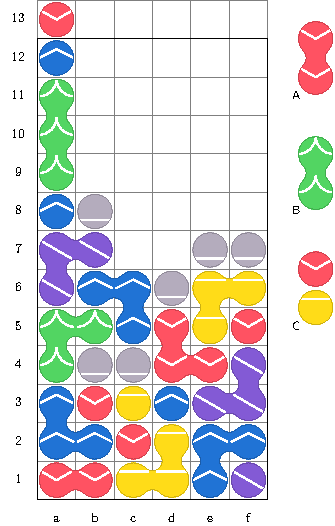
\includegraphics{subfigures/cover_big_board.pdf}
\end{halfpage}%
\begin{halfpage}[Puyo\tex]
	A \latex package for quickly typesetting board states of Puyo Puyo games.\parlineskip
	Supports large and small boards with arbitrary shape, hidden rows, current and next puyos, labels and move planning markers.\parlineskip
	Source code available for download on \github or your favorite \tex repository. Package requires \python in support of scripts driven by \pythontex.\parlineskip
	Move planning markers shown at left. Tailing variations on the Great Tanaka Rensa (GTR) shown below.\parlineskip
	Created by \link{https://twitter.com/terramyst1}{terramyst}.
\end{halfpage}

\parline
\noindent
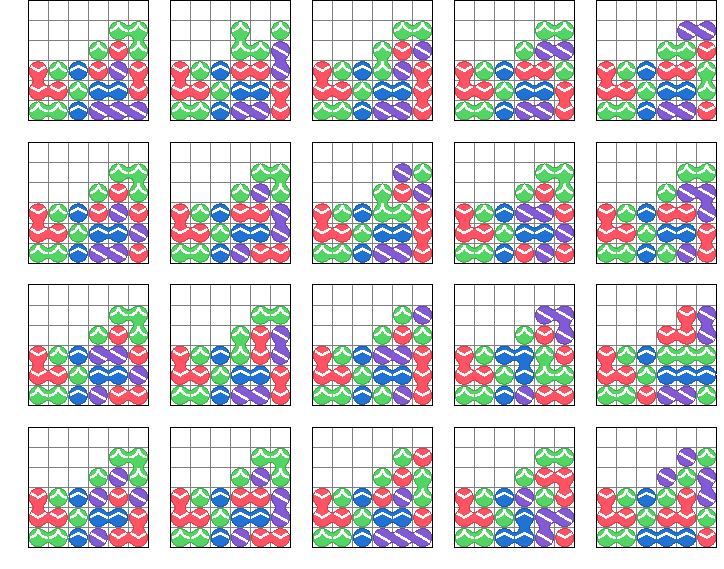
\includegraphics{subfigures/cover_small_boards.pdf}

\section{Installation}
\subsection{Python3 and PythonTeX}
Installing this package should be straightforward through the user's \tex package manager. \python will additionally need to be installed; it is recommended to use a virtual environment management tool such as \anaconda. The Python environment will need packages \pypygments and \pynumpy installed.\par
Compiling the document requires inserting a new command into the build sequence. \pythontex must run \code{pythontex.py} in between two separate runs of the \tex engine (see documentation for more detail).

\section{Usage}
This package provides an environment and three macros for typesetting Puyo Puyo boards for inclusion in \latex documents.

\codepar{puyotikz}{environment}
The \code{puyotikz} environment is simply a wrapper for the \code{tikzpicture} environment. The user is therefore able to use additional \tikzpgf macros inside this environment if they wish to augment whatever graphics are already provided by this package.\par
The \code{puyotikz} environment takes a single numeric argument which is passed to the \code{tikzpicture} environment as the scaling parameter. This package provides two scaling parameter definitions for convenience, \cmd{puyosmallscale} and \cmd{puyobigscale} (the default).

\begin{puyolisting}
	% example usage
	\begin{puyotikz}[\puyosmallscale]
		% content... 
	\end{puyotikz}
\end{puyolisting}

For the traditional colors of red, yellow, green, blue, purple, and gray this package also provides new color definitions such as \code{bluepuyo} and \code{darkredpuyo}.

\pagebreak
\codepar{puyoboard}{macro}
The \cmd{puyoboard} macro takes 2 arguments and 4 optional parameters and must be used inside the \code{puyotikz} environment.\par
Puyos are specified in format strings by column (bottom-up, left-to-right). Each puyo is identified by a single letter (\code{r}, \code{y}, \code{g}, \code{b}, \code{p}, \code{n}). Columns (or next puyos) are separated by \code{/}. Columns are labeled numerically and rows and next puyos are labeled alphabetically (lowercase and uppercase, respectively).

\begin{puyolisting}
	% parameters
	%	- ncols: number of columns (default 6)
	%	- nrows: number of visible rows (default 12)
	%	- nhidrows: number of hidden rows (default 1)
	%	- showlabels: display coordinate labels (default True)
	
	% arguments
	%	- #1: board format string
	%	- #2: next puyos format string
	
	% example usage (see image above)
	\begin{puyotikz}
		\puyoboard[ncols=12, nrows=6, nhidrows=0]
			{/rr/brbb/ggbg/rrg//yb/ggy}
			{yy/yr}
	\end{puyotikz}
\end{puyolisting}

\begin{center}
	\begin{puyotikz}
		\puyoboard[ncols=12, nrows=6, nhidrows=0]
			{/rr/brbb/ggbg/rrg//yb/ggy}
			{yy/yr}
	\end{puyotikz}
\end{center}

\pagebreak
\codepar{puyomarker}{macro}
The \cmd{puyomarker} macro takes 1 argument and must be used inside the \code{puyotikz} environment following a \cmd{puyoboard} macro.

Puyo markers are specified in a single format string, separated by \code{/}. A single marker is a concatenation of the row label (lowercase letter), column label (number), puyo color (lowercase letter) and puyo label (uppercase letter).

\begin{puyolisting}
	% arguments
	%	- #1: marker format string
	
	% example usage (see image above)
	\begin{puyotikz}
		\puyoboard[ncols=12, nrows=6, nhidrows=0]
			{/rr/brbb/ggbg/rrg//yb/ggy}
			{yy/yr}
		\puyomarker{a1yA/a2yA/b3yB/b4rB}
	\end{puyotikz}
\end{puyolisting}

\begin{center}
	\begin{puyotikz}
		\puyoboard[ncols=12, nrows=6, nhidrows=0]
			{/rr/brbb/ggbg/rrg//yb/ggy}
			{yy/yr}
		\puyomarker{a1yA/a2yA/b3yB/b4rB}
	\end{puyotikz}
\end{center}

\pagebreak
\codepar{puyogrid}{macro}
The \cmd{puyogrid} macro is provided as an example derived from \cmd{puyoboard}. It assumes a \cmd{puyosmallscale} \code{puyotikz} environment and only provides a single argument for the board format string (assuming no next puyos and no markers). It also assumes zero hidden rows and turns off labeling, however any parameters available to set in \cmd{puyoboard} are also available in \cmd{puyogrid}.\par
The user is encouraged to construct their own derived macros in similar fashion for their intended purpose.

\begin{puyolisting}
	% source code \puyogrid definition from puyotex.sty
	\newcommand{\puyogrid}[2][]{
		\setkeys{puyoboard}{nhidrows=0, showlabels=False}
		\begin{puyotikz}[\puyosmallscale]
			\puyoboard[#1]{#2}{}
		\end{puyotikz}
	}

	% example usage
	\puyogrid[nrows=4, ncols=10]
		{rrr/yyyr/gggy/bbbg/pppb/rrrp/yyyr/gggy/bbbg/pppb}
\end{puyolisting}

\begin{center}
	\puyogrid[nrows=4, ncols=10]{rrr/yyyr/gggy/bbbg/pppb/rrrp/yyyr/gggy/bbbg/pppb}
\end{center}

\section{Limitations}

\subsection{TikZ}
The graphics provided in this package are created using \tikzpgf. Having many graphics compiled in a single document will result in a long compilation time.\par
It is recommended in this case to generate images in separately compiled standalone documents and include them in the main document via \cmd{includegraphics}. \pythontex is not compatible with \cmd{tikzexternalize}.

\subsection{PythonTeX}
The \pythontex documentation gives a warning which bears repeating: compiling a document that uses \pythontex involves executing Python code on your computer therefore you should only compile documents from sources you trust.

\end{document}